\subsubsection{Pemodelan, Penyimpanan, dan \textit{Indexing} Data Smart Contracts}

% jadi bahas alternatif dulu, misal yang terpilih eth2dgraph
% lalu bahas schema yang dipakainya gimana, yang base nya apa aja secara singkat, dan yang mau ditambahinnya apa, berdasarkan apa
% Jadiin dua subheading

\begin{figure}[ht]
	\centering
	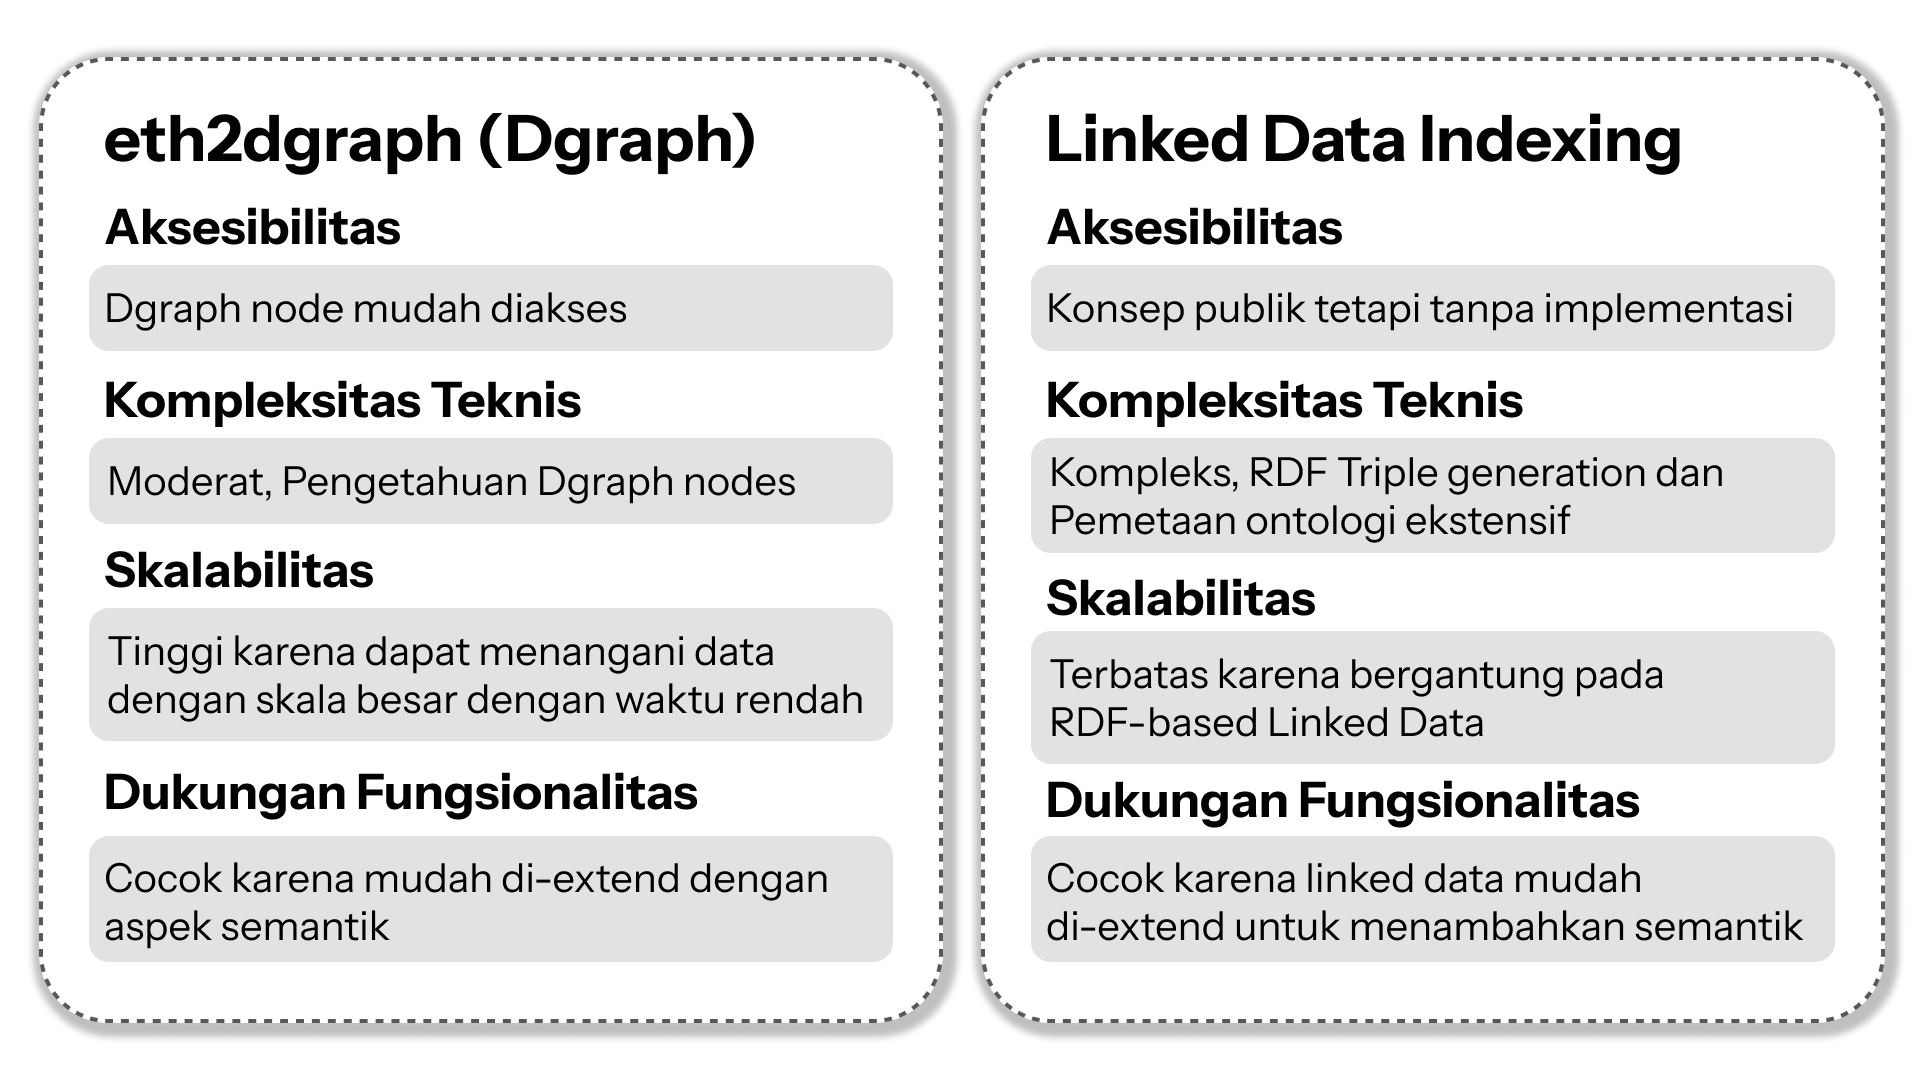
\includegraphics[width=0.7\textwidth]{resources/chapter-3/pemodelan-1.png}
	\caption{Perbandingan alternatif pemodelan, penyimpanan, dan \textit{indexing} data Smart Contracts}
	\label{image:pemodelan-1}
\end{figure}

\begin{figure}[ht]
	\centering
	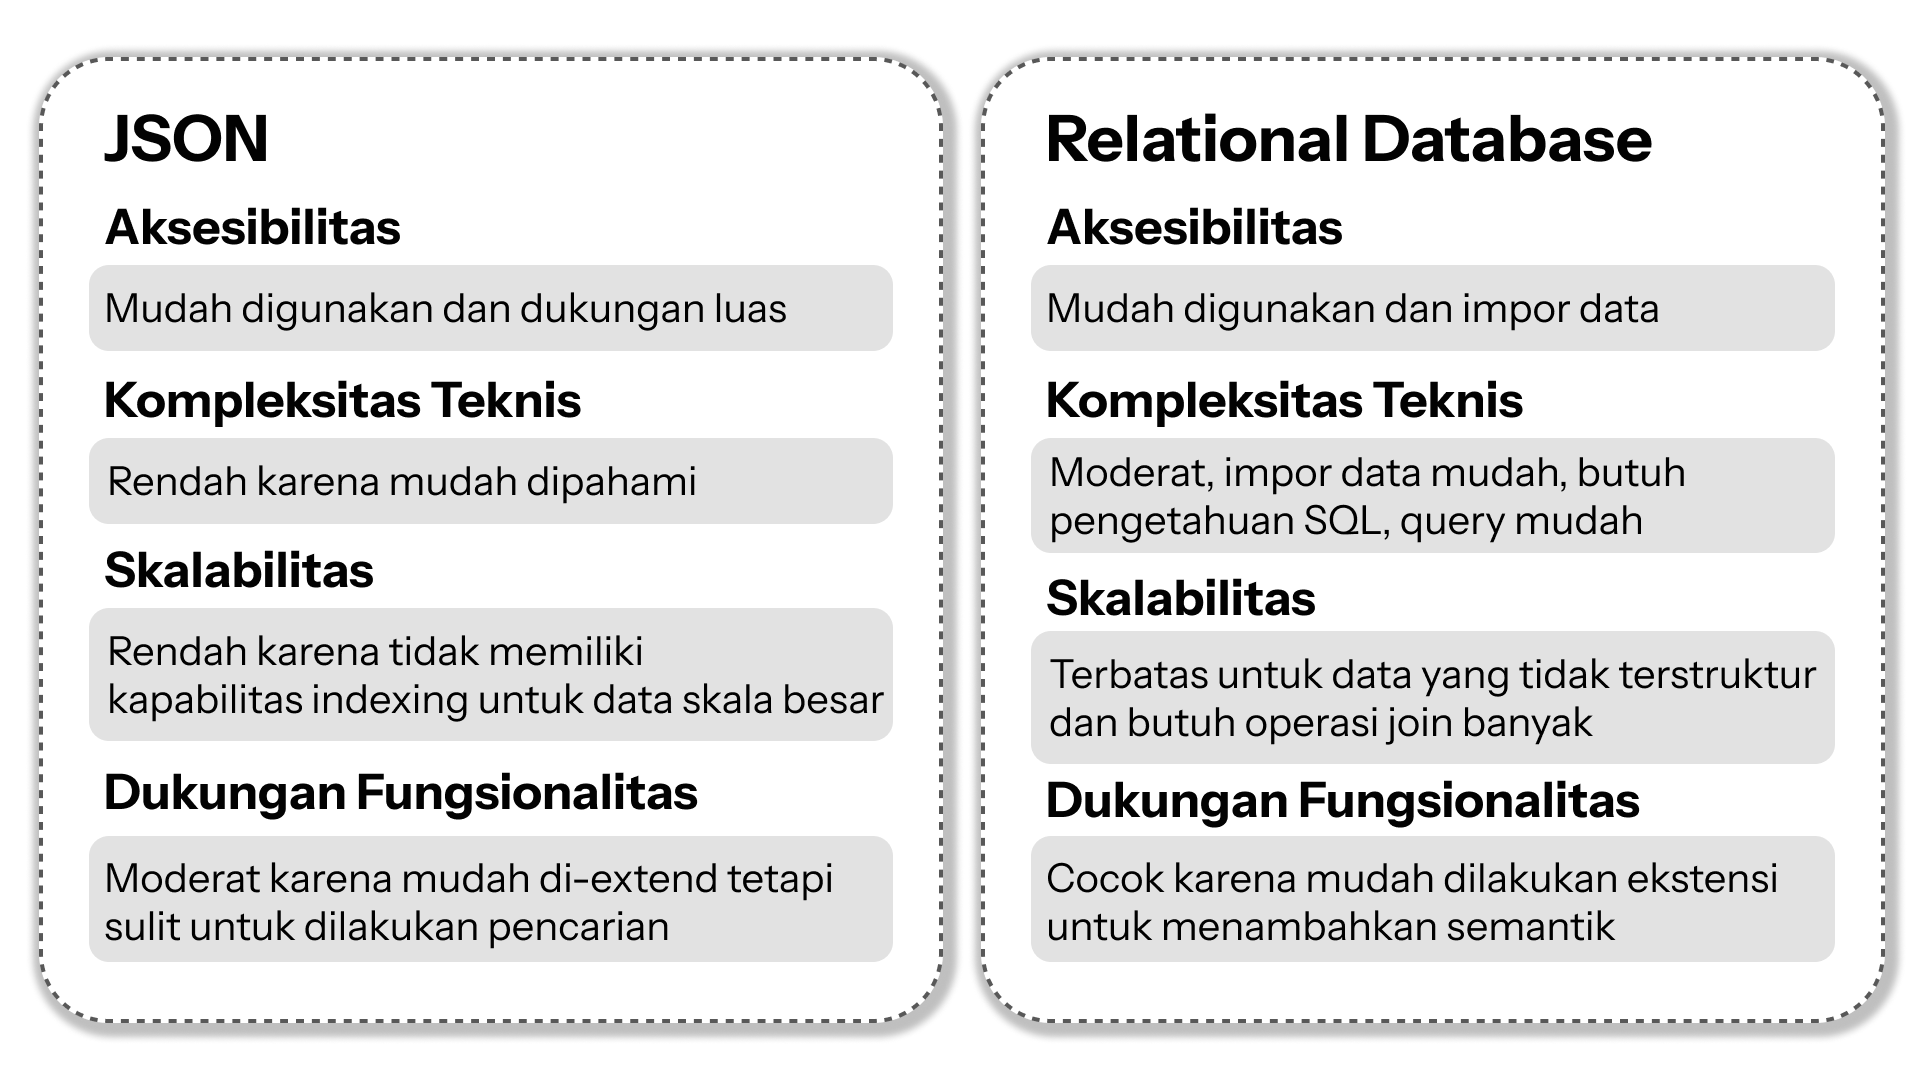
\includegraphics[width=0.7\textwidth]{resources/chapter-3/pemodelan-2.png}
	\caption{Perbandingan alternatif pemodelan, penyimpanan, dan \textit{indexing} data Smart Contracts}
	\label{image:pemodelan-2}
\end{figure}

Data yang diekstrak dari Blockchain Ethereum perlu dimodelkan, disimpan, dan di-\textit{indexing} agar dapat diakses dengan efisien. Secara fungsional, untuk pemodelan, dibutuhkan ekstensibilitas yang baik untuk model, sehingga dapat menampung data yang lebih banyak dan lebih kompleks. Untuk penyimpanan, dibutuhkan skalabilitas yang baik untuk menyimpan data yang besar, serta dukungan untuk melakukan query dengan efisien. Untuk \textit{indexing}, dibutuhkan kemampuan untuk melakukan query dengan cepat dan efisien.

Berikut merupakan beberapa alternatif yang dapat digunakan untuk pemodelan, penyimpanan, dan \textit{indexing} data Smart Contracts:
\begin{enumerate}
	\item \textbf{eth2dgraph (Dgraph)} \parencite{aimar2023extraction} (Bagian \ref{subsec:extraction-indexing-analysis-ethereum-sc}): Selain digunakan untuk ekstraksi data, riset ini juga menyediakan pemodelan, penyimpanan, dan \textit{indexing} data Smart Contracts menggunakan Distributed Graph Database. Keunggulannya adalah penggunaan Dgraph yang memiliki kemampuan skalabilitas tinggi dan dapat melakukan query dengan efisien. Secara aksesibilitas, Dgraph mudah diakses dengan 3 node utama, ratel, zero, dan alpha, yang dapat dijalankan secara lokal. Secara kompleksitas, eth2dgraph tergolong moderat karena memerlukan pengetahuan dasar tentang Dgraph nodes dan pemodelan graf. Namun, Dgraph memiliki dokumentasi yang baik dan komunitas yang aktif, sehingga memudahkan pengguna dalam memahami dan menggunakan teknologi ini. Dalam hal dukungan fungsional, format dgraph dapat di-\textit{extend} dengan mudah untuk menambahkan aspek semantik yang dapat membantu dalam pencarian Smart Contracts.

	\item \textbf{Linked Data Indexing of Distributed Ledgers (Linked Data)} \parencite{third2017linked} (Bagian \ref{subsec:linked-data-indexing-distributed-ledgers}): Riset ini menerapkan indeks semantik pada data Blockchain menggunakan Linked Data dengan keunggulan penggunaan ontology BLONDiE dan MSM untuk mendeskripsikan semantik Smart Contracts dan fokus pada aspek \textit{discoverability}. Secara aksesibilitas, konsep riset ini \textit{public}, namun tanpa implementasi \textit{open source}. Implementasinya kompleks karena memerlukan pemetaan ontology ekstensif dan RDF triple generation, tanpa dukungan \textit{tools} atau \textit{framework}. Skalabilitas riset ini terbatas karena bergantung pada RDF-based Linked Data, yang kurang cocok untuk data Blockchain besar. Secara dukungan fungsional, walaupun format linked data dapat dengan mudah di-\textit{extend} untuk menambahkan aspek semantik yang dapat membantu dalam pencarian Smart Contracts.

	\item \textbf{JSON}: Merupakan format data yang umum digunakan untuk menyimpan dan mentransfer data. JSON memiliki keunggulan dalam kemudahan penggunaan dan dukungan luas di berbagai bahasa pemrograman. Namun, JSON tidak memiliki kemampuan \textit{indexing} yang efisien untuk data besar, sehingga kurang cocok untuk sistem yang memerlukan skalabilitas tinggi. Secara kompleksitas, JSON tergolong rendah karena mudah dipahami dan digunakan, serta dapat dilakukan ekstensi dengan baik.

	\item \textbf{Relational Database (SQL)}: Merupakan sistem basis data yang menggunakan model relasional untuk menyimpan data. SQL memiliki keunggulan dalam kemampuan \textit{indexing} dan query yang efisien untuk data besar. Namun, SQL memiliki keterbatasan dalam hal fleksibilitas dan skalabilitas untuk data yang tidak terstruktur atau semi-terstruktur. Secara kompleksitas, SQL tergolong moderat karena memerlukan pengetahuan dasar tentang basis data relasional dan bahasa query SQL. Secara dukungan fungsional, SQL dapat di-\textit{extend} dengan baik untuk menambahkan aspek semantik yang dapat membantu dalam pencarian Smart Contracts.
\end{enumerate}

Secara singkat, keempat alternatif ini dapat disimpulkan dengan diagram-diagram pada gambar \ref{image:pemodelan-1} dan gambar \ref{image:pemodelan-2}.